\subsubsection{DNA replication}

During exponential growth, the cell needs to duplicate its DNA content in order to proceed to division. Replication of DNA needs to be well coordinated with cell growth and division to ensure viability of the daughter cells. There are three important phases: replication initiation, elongation and termination. These phases are controlled by several (partly unknown) mechanisms to adapt to external conditions and adjust growth rate. For example, several bacteria, including \textit{E. coli} and \textit{B. subtilis}, are able to initiate replication several times during one cell cycle, so that the cell cycle can actually be shorter than the time needed to replicate the full chromosome \citep{reyes-lamothe_chromosome_2012}.

\paragraph{Replication initiation} Replication initiation of the chromosome is an event that appears to be precisely controlled. Replication should only be initiated if growth conditions are favorable. What is more, replication should not be triggered several times during cell cycle (except in excellent growth conditions), implying the existence of mechanisms that inhibit replication initiation once replication has already started.

Initiation is mainly controlled by DnaA, a protein that can bind DNA in its activated form, DnaA-ATP. There are numerous DnaA binding boxes along the chromosomes, but only a few of them are essential for replication initiation. The latter are located next to the \textit{oriC} locus (Figure \ref{fig:dnaA}, top), where the replisomes are loaded and replication actually starts. Interestingly, \textit{oriC} and the \textit{dnaA} gene are colocated in numerous bacteria \citep{briggs_chromosomal_2012}, so that the binding of DnaA inhibits its own expression, autoregulating the levels of DnaA available.

When it is activated, DnaA polymerizes along the DnaA binding boxes, unwinding the DNA around \textit{oriC}. It is probable that this unwinding is not necessarily performed by DnaA itself. For example, in \textit{B. subtilis}, DnaA binds with DnaD, which is mainly responsible for untwisting \citep{briggs_chromosomal_2012}. Once the DNA is sufficiently untwisted, a neighboring AT-rich region, termed DNA-Unwinding Element (DUE), opens slightly, enabling loading of the first elements of the replisomes, the helicase and helicase loader (DnaC-DnaI for \textit{B. subtilis}, DnaB-DnaC for \textit{E. coli}). The position of DnaA binding boxes is not exactly conserved in different bacterial species, the loading mechanism is poorly understood. Because a loop is observed during replication initiation of \textit{B. subtilis}, \citet{briggs_chromosomal_2012} propose that DnaD is used for loop-forming and that the loop enables synchronous loading of the two replisomes (one for each direction) through DnaB (Figure \ref{fig:dnaA}, bottom).

\begin{figure}[!ht]
	\centering
	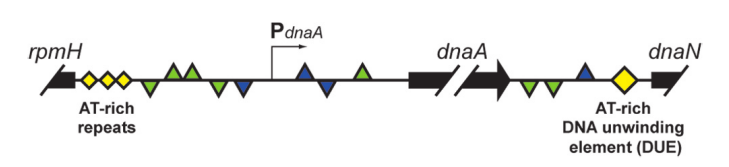
\includegraphics[width=0.8\linewidth]{figure/dnaABindingBoxes}
	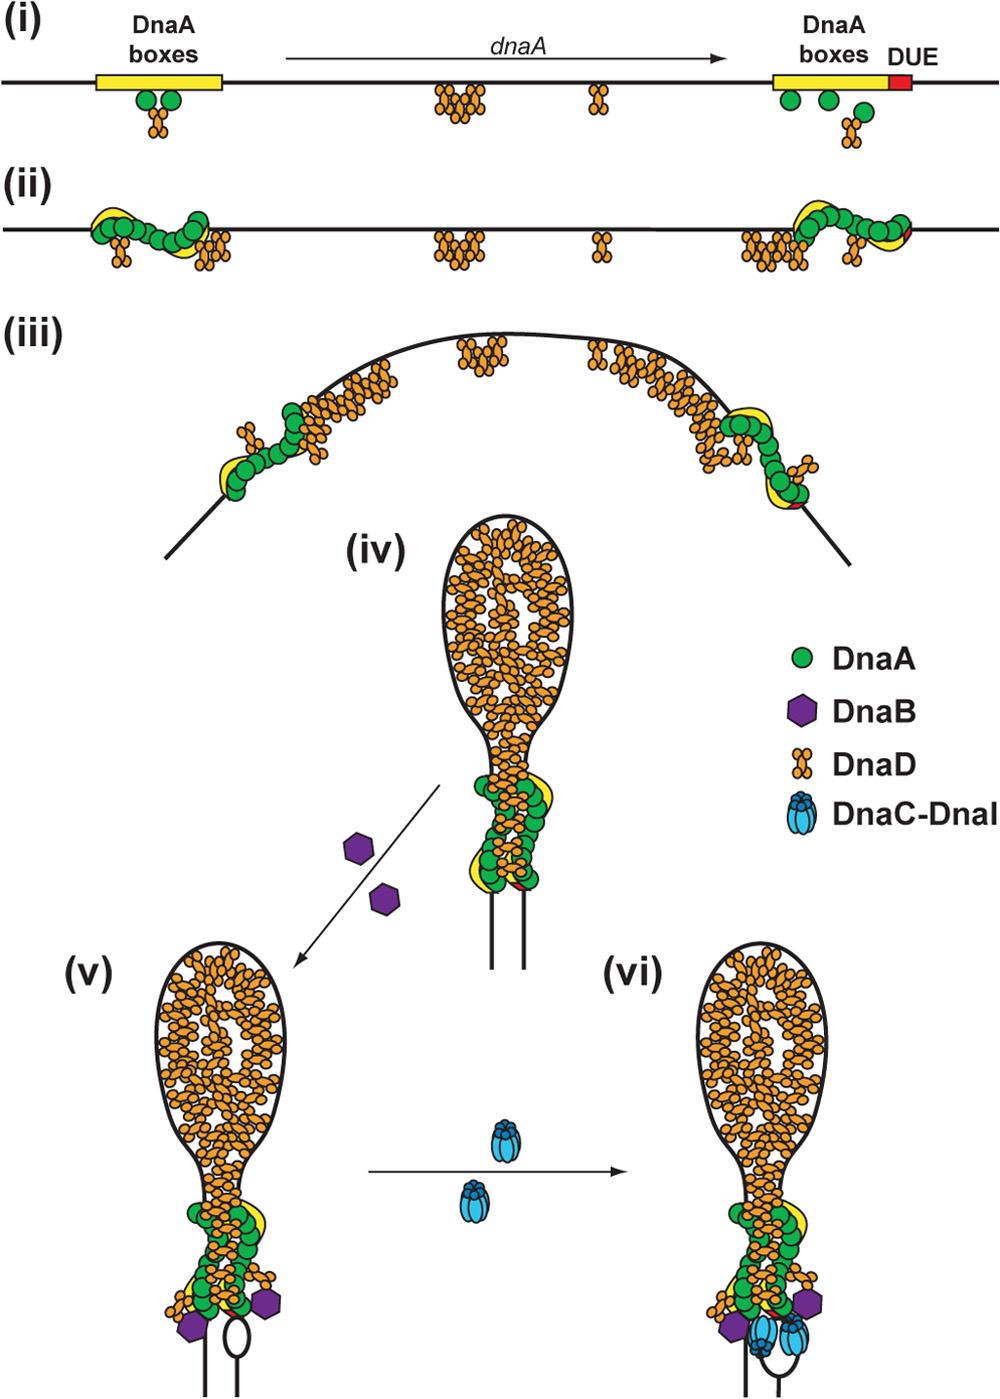
\includegraphics[width=0.5\linewidth]{figure/dnaAPolymerizationModel}
	\caption{Control of DNA replication through DnaA proteins and other helper proteins in \textit{B. subtilis}. Around \textit{oriC}, several DnaA binding sites (blue and green triangles) allow for the polymerization of DnaA and, eventually, opening of the DNA at the AT-rich DNA-Unwinding Element (DUE) (top). Model for replisome loading by helper proteins (bottom). DnaD accelerates DnaA binding and its unwinding and polymerization activities form a loop. Finally DnaB is recruited on each end on the loop, each DnaB loading a helicase DnaC on one of the strands with the help of helicase-loader DnaI. Figures from \citet{briggs_chromosomal 2012}.}
	\label{fig:dnaA}
\end{figure}
How initiation is controlled is largely unknown. For example, \textit{E. coli} does not have homologs for \textit{B. subtilis} DnaB and DnaD proteins (\textit{E. coli} DnaB and DnaC are the homologs of \textit{B. subtilis} DnaC and DnaI, respectively). As a result, the initiation is strongly dependent on DnaA-ATP levels in \textit{E. coli} but less in \textit{B. subtilis}, where DnaB and DnaD seem more critical \citep{briggs_chromosomal_2012}. In any case, decreasing DnaA-ATP levels by hydrolysis seems to be an efficient way to prevent initiation. This seems to be one of the strategies to avoid immediate reinitiation. The replisome contains processivity $\beta$-clamps (see below), that bind to proteins that hydrolize DnaA-ATP. What is more, once replication has started, the number of DnaA binding sites rapidly increases, diluting remaining DnaA-ATP. The concentration of DnaA-ATP may increase again when DnaA is newly synthesized. Another possible mechanism for initiation control is the ParAB-\textit{parS} system \citep{reyes-lamothe_chromosome_2012}. This system, probably responsible for chromsome segregation (see below), binds to the \textit{parS} locus through parB. It seems that ParA binds DnaA and influences replication initiation, maybe because ParB hydrolyzes ParA, complexing ParB-\textit{parS} to the \textit{oriC}, this association being stabilized by SMC proteins. The complex can then migrate towards one of the cell poles and it is possible that it may be unavailable for reinitiation during that time.

Even though our understanding of the initiation of replication on the chromosome is limited, experiments show that it is strictly controlled by the cell. On the other hand, the replication of other DNA elements such as plasmids is not as severely controlled, as their exact number within the cell can vary. Initiation is not triggered by DnaA but by other proteins or RNAs that are plasmid-specific. Shortly, there are two main types of plasmids in a bacterial cell: large plasmids present in low copy numbers and small plasmids present in high copy numbers (Figure \ref{fig:plasmidInitiation}). The large plasmids have a similar initiation system as the chromosome, triggered by a DNA binding protein coded by the plasmid itself (generically called Rep). Initiation is probably regulated by the copy number of plasmids, either through a RNA coded by the plasmid that blocks the synthesis of Rep, or simply because Rep is able to polymerize at high concentrations, becoming unavailable for initiation. In small plasmids, initiation is probably controlled by a RNA and DNA polymerase I. The RNA (termed RNAII) slightly opens the double helix and binds to DNA, acting as a primer for DNA polymerase I, which further opens DNA. A single replisome can then be loaded on the other strand (in this case, replication is unidirectional). Copy number is probably controlled by another RNA (termed RNAI), which interfers with RNAII at sufficiently high concentrations.

\begin{figure}[!ht]
	\centering
	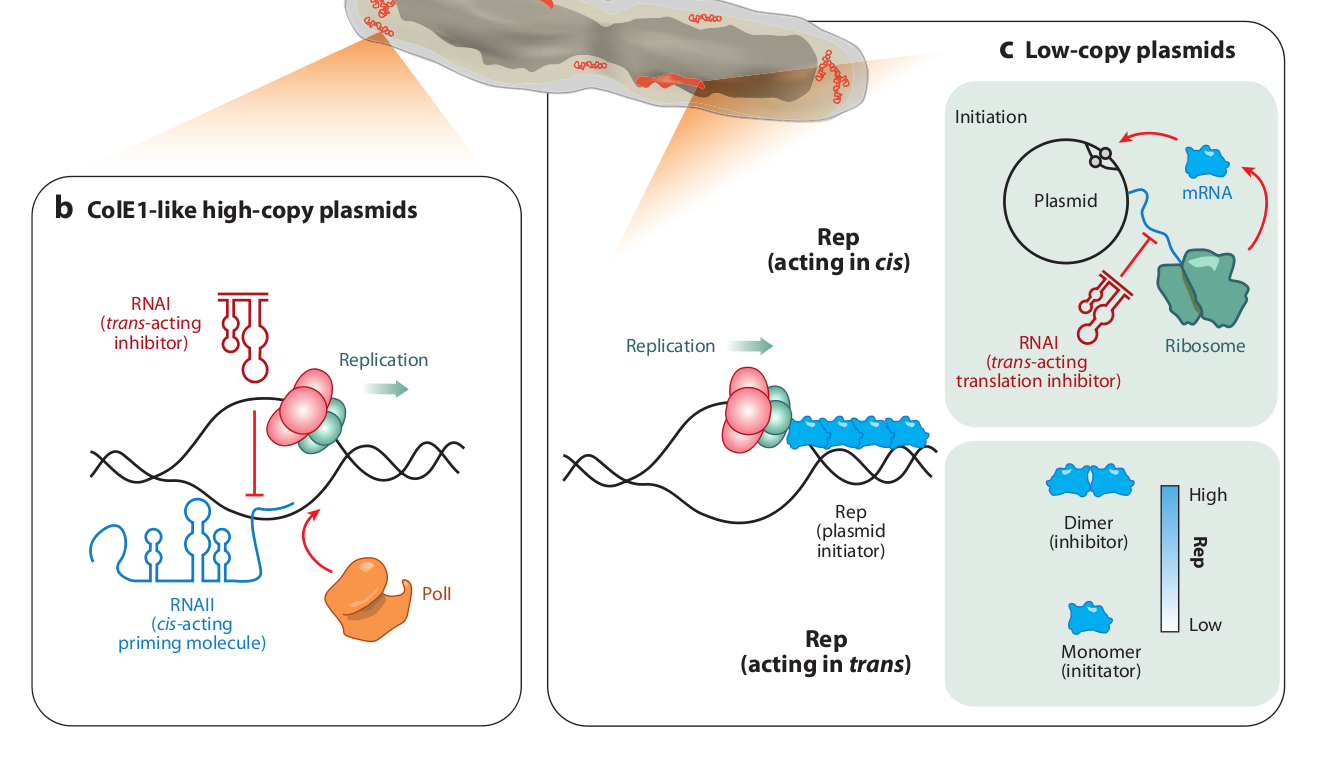
\includegraphics[width=0.8\linewidth]{figure/plasmidReplicationInitiation}
	\caption{Plasmid replication follows similar principles as chromosome replication (it uses the same replisome). However, initiation is regulated by plasmid specific elements. Small plasmids probably use RNAs to initiate (RNAII) and inhibit (RNAI) replication. Large plasmids use a protein that acts similarly to DnaA and which is regulated by the plasmid copy number. Figure from \citet{reyes-lamothe_chromosome_2012}}.
	\label{fig:plasmidInitiation}
\end{figure}

\paragraph{Replication elongation} Once replication is initiated, helicases are loaded upon the DNA strands, one in each direction (see above). From the helicases, the whole replisome complex can be loaded and start polymerizing DNA. The replisome ensures processivity and rapid replication of the whole chromosome, as well as synchronous replication of the leading strand and the lagging strand. Indeed, DNA polymerases are only able to assemble DNA in the 5' to 3' sense, which corresponds to the direction the leading strand is processed, but antisense to lagging strand processing. Therefore, the leading strand is easily handled while replication of the lagging strand is handled by loop forming that allows for fragment-wise replication of a few kbs of DNA (termed Okazaki fragment).

The composition of the replication reflects these different tasks (Figure \ref{fig:replisome}). The helicase DnaB (DnaC for \textit{B. subtilis}) is formed of a hexamer that separates the DNA, forming the replication fork. Bound to the helicases, three primases DnaG stabilize the helicase structure and cooperate for synthesis of short RNA sequences on the lagging strand called primers used to initiate Okazaki fragments. Finally, a clamp loader bound to the helicase is responsible for recruiting DNA polymerases and $\beta$-clamps. The number of DNA polymerases can vary depending on the number of subunits $\tau$ in the clamp loader \citep{reyes-lamothe_chromosome_2012,stratmann_dna_2014}: replisomes with 2 or 3 associated DNA polymerases have been observed, the latter seemingly more efficient. The nature of DNA polymerases is also unclear: it seems that in \textit{E. coli} Pol III is preferentially recruited because of its high fidelity, while in \textit{B. subtilis} two different polymerases may be used for the leading and the lagging strand \citep{reyes-lamothe_chromosome_2012,stratmann_dna_2014}. The recruitment of $\beta$-clamps is also essential as it binds to DNA polymerases and increases their processivity from a few nucleotides to several tenths of kb \citep{reyes-lamothe_chromosome_2012}. Because these elements are bound to the clamp loader, they are efficiently recycled, allowing for very fast replication.
\begin{figure}[!ht]
	\centering
	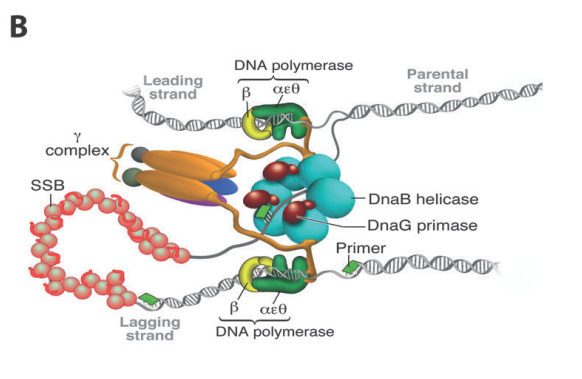
\includegraphics[width=0.6\linewidth]{figure/replisome}
	\caption{Standard bacterial replisome stucture (as reconstructed from \textit{E. coli}). Figure from \citet{stratmann_dna_2014}.}
	\label{fig:replisome}
\end{figure}

Coordination of leading and lagging strand replication is not fully understood. As replication occurs continuously on the leading strand, it seems intuitive that replication should occur more rapidly than on the lagging strand or that the loop forming/relase of Okazaki fragments has to be particularly efficient. Two models have been proposed for the loop forming process: the collision process and the signaling process (Figure \ref{fig:replisomeElongation}, left). In both models, DNA polymerase starts from a primer, progressively forming a loop as ssDNA (protected by SSB) and recently polymerized DNA accumulate between the fork and the DNA polymerase. In the collision model, the DNA polymerase proceeds until the next Okazaki fragment, stalling and becoming available for elongation from the next primer. If a primer is ready before the current fragment is finished, the fork could pause, making this process quite inefficient. In the signalling model, the DNA polymerase is reused as soon as a primer is ready, so that a lot of fragments remain incomplete, containing large portions of ssDNA. In fact, the presence of 3 polymerases indicates that the reality might be in-between, explaining how the lagging strand synthesis can be as efficient as the leading strand synthesis (Figure \ref{fig:replisomeElongation}) \citep{stratmann_dna_2014,duderstadt_replication-fork_2014}. With 3 polymerases, 2 polymerases might be synthesizing at the same time, one finishing the previous fragment while the other one is available for recruitment on a new primer. As a matter of fact, it is also highly probable that the replisome is very dynamic, with frequent recruitment and detachment of primases and polymerases. In this way, even a 2 polymerase replisome could operate in a similar manner, by periodically detaching polymerases to finish a fragment and recruiting a new polymerase at the replisome. This remains to investigate but seems pretty likely as numerous polymerases gravitate around the replisome and such exchanges have been observed on the leading strand \citep{stratmann_dna_2014}.
\begin{figure}[!ht]
	\centering
	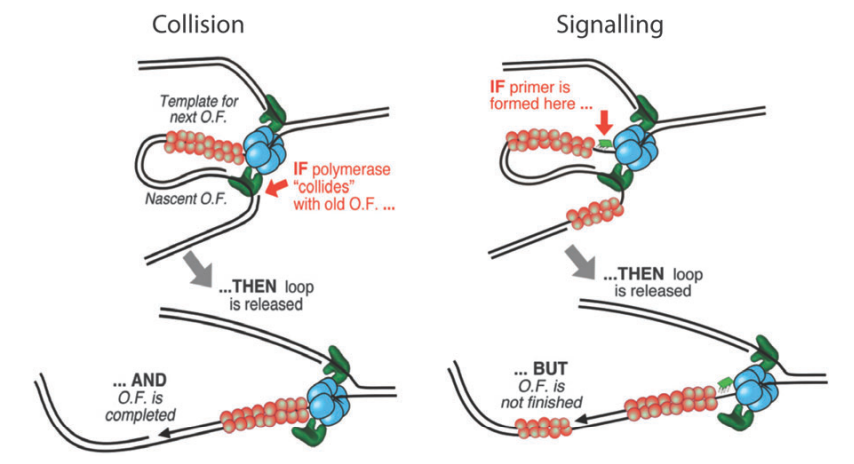
\includegraphics[width=0.49\linewidth]{figure/replisomeElongation}
	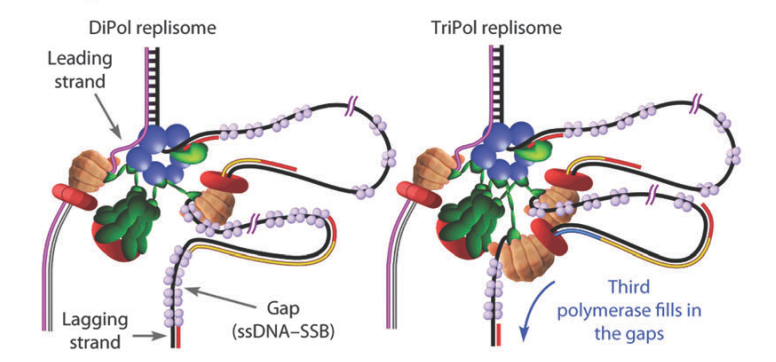
\includegraphics[width=0.49\linewidth]{figure/replisomeThreePolymerases}
	\caption{Elongation models for the lagging strand (left). Likely elongation according to recent experiments that mixes the two previous models (right). Figure from \citet{stratmann_dna_2014}.}
	\label{fig:replisomeElongation}
\end{figure}

Some details of elongation remain unclear. RNA primers have to be removed, resynthesized and ligated by specific polymerases, but the coordination with the replisome has not been investigated (to our knowledge). The cooperation with SMC molecules or obstacle management is known to exist but very little is known. Some elements are presented in the repair section, where stalling of the replisome is handled by RecA and restarting of replication is handled by a specific primosome complex. However, it is unknown if the replisome collapses, helps recruiting repair proteins or lower fidelity polymerases that can bypass some specific DNA damages.

\paragraph{Replication termination} Termination of replication occurs in the \textit{terC} region thanks to Tus proteins. These proteins are able to block a replisome along one direction. Replisomes will thus meet along a small segment delimited by two Tus proteins in opposite directions, probably even at the site of one of these proteins. The length of the two replicons is thus not totally fixed but limited to a certain range.


\paragraph{Computational representation}
See illustration how the cell chromosome is used. Some more information may be needed TBD.
When a chromosome is fully duplicated (when the first column of the cell chromosome only contains -2), the process consists of deleting the current chromosome and creating 2 new ones with the correct initialization. TBD do we clean the chromosomes? Typically, when the chromosome was manipulated.

Needs also other things but from the DNA point of view, there seems to have enough information.

\subsubsection{DNA movement}
\textcolor[rgb]{1.00,0.00,0.00}{What do we do when a gene change of volume due to condensation or segregation for example. Normally, a matter of changing the number of the volume in the cell chromosome and the corresponding volume chromosomes. But assume that anything that is currently binded to the DNA is the property of the DNA and was 'erased' from everywhere else. Also assume that volume chromosome only contains the strictly necessary information about the DNA in the volume and that it is a state with changing size.}

\subsubsection{DNA manipulations}
\paragraph{Codon aggregation damage}
\textcolor[rgb]{1.00,0.00,0.00}{Gap site, Abasic site, Sugar-phosphate, Base, Intrastrand cross link, Strand break, Holliday junction}
DNA is subject to numerous forms of damage that can be either endogenous or exogenous. They can result in chemical modifications of some bases, in single strand breakage (missing of one base on one of the strands), double strand breakage or cross links between DNA strands. Chemical modifications can originate from different type of radiations (UV, x-rays, etc.), drugs or reactants naturally present in the cell leading to alkylations, oxydations, deaminations, etc. Another important source of DNA mismatches is the replication machinery itself which can make use of the wrong dNTP (dUTP for example).

DNA modification is one of the prerequisites to evolution. DNA mutations lead to the development of novel functions, regulatory systems, etc. However, replication fidelity is also essential for selection and conservation of important existent functions. There is a trade-off between these two aspects that is well illustrated in \textit{B. subtilis} by the existence of efficient repair mechanism on the one hand and some DNA polymerases that favor propagation of some types of damage (such as DnaE) on the other hand.



\paragraph{Codon aggregation insertion}
Insertion of one (or several) lines in the DNA states.

\paragraph{Codon aggregation deletion}
Putting 0 in the corresponding places and not deletion of the line(s) because a codon aggregation can be deleted in a fork.

\paragraph{Codon aggregation repair}
There are several pathways employed for DNA repair corresponding to the type of damage undergone.

\subparagraph{Mismatch Repair (MMR)} This pathway is dedicated to reparation of base mismatches. In \textit{E. coli}, repairing is initiated by MutS (Sensor) which detects the mismatch and MutL (Linker) which recruits further proteins. The endonuclease MutH then nicks the DNA next to the mismatch enabling the helicase and exonuclase UvrD to remove bases around the mismatch. The resulting gap is filled in by DNA polymerase III and DNA Ligase. The newly synthesized strand is specifically targeted by these proteins thanks to the methylase Dam used for marking the original strand. In \textit{B. subtilis}, only MutS and MutL seem to be conserved (MutL having an additional endonuclease activity). Recognition of the newly synthesized strand could be linked to a strong coupling of MMR with replication and colocalization with the replisome.

\subparagraph{Base excision repair (BER)} The BER pathway repairs most non-bulky base modifications such as oxydations, deaminations, UTP incorporation, etc. Schematically, glycosylases detect the lesion, remove the damaged base, endonucleases then nick the DNA next to the missing base so that exonucleases remove some bases on the strand around the missing base. The small gap is then closed by a repair DNA polymerase (such as Polymerase I) and ligated by a DNA ligase. For example, in \textit{B. subtilis}, the glycosylases MutM and MutY (part of the GO system) detect oxidized Guanine to avoid its pairing up with dATP. Another example is Uracil DNA-glycosylase, which removes dUMP from DNA. 

\subparagraph{Nucleotide excision repair (NER)} The NER pathway is very similar to the BER pathway, except that it repairs bulky lesions caused by UV radiations or drugs. This pathway is highly conserved and partly regulated by the SOS response (mediated by RecA). The UvrABC complex is responsible for detecting the damaged base and nicking the DNA at surrounding bases. Helicase UvrD removes the nicked segment. Finally, DNA Pol. I and DNA ligase restore the missing segment.

\subparagraph{Alkylation damage} There are specific pathways that address alkylation (such as methylations). \textit{B. subtilis}, as a soil-living bacterium, is particularly exposed to alkylating agents. There are at least three pathways responsible for repairing alkylated bases: two pathways based on glycosylases (one being constitutive, the other inducible) and one pathway based on alkyltransferases (enzymes that suicide by transferring the alkyl group onto themselves).

\subparagraph{Homologous recombination (HR)} During replication, double strand breaks (DSB) can be repaired by using the other copy of the chromosome (Figure \ref{fig:HR}). First, the DSB is stabilized by RecN and digested by protein complexes (AddAB and RecQSJ in \textit{B. subtilis}) that create hangovers of single stranded DNA (ssDNA) on the 3' strands. RecA binds to the ssDNA (probably with the help of the RecFOR complex that prevents SSB from binding). RecA, activated by ATP or dATP, enables invasion of the sister chromosome at a homologous sequence, creating a D-loop where one of the broken 3' strands is inserted and forming Holliday Junctions between the two chromosomes. DNA elongation occurs from the 3' strand and the Holliday Junctions are cleaved by RecU (or a homologous protein).

There is a variation if the DSB caused the replication to stall (Figure \ref{fig:HR}, right). This situation may occur if a single-strand break is present on the original chromosome which becomes a DSB after passage of the replication fork. In this case, there is only one DNA end to digest and the invasion leads to only one Holliday Junction. The primosome complex, composed of Pri and Dna proteins, detects the D-loop and helps loading the replisome to resume replication. It seems that several Structural Maintenance of Chromosome (SMC) proteins are involved throughout the process (such as RecN), but their role is not clearly elucidated.

\begin{figure}[!ht]
\centering
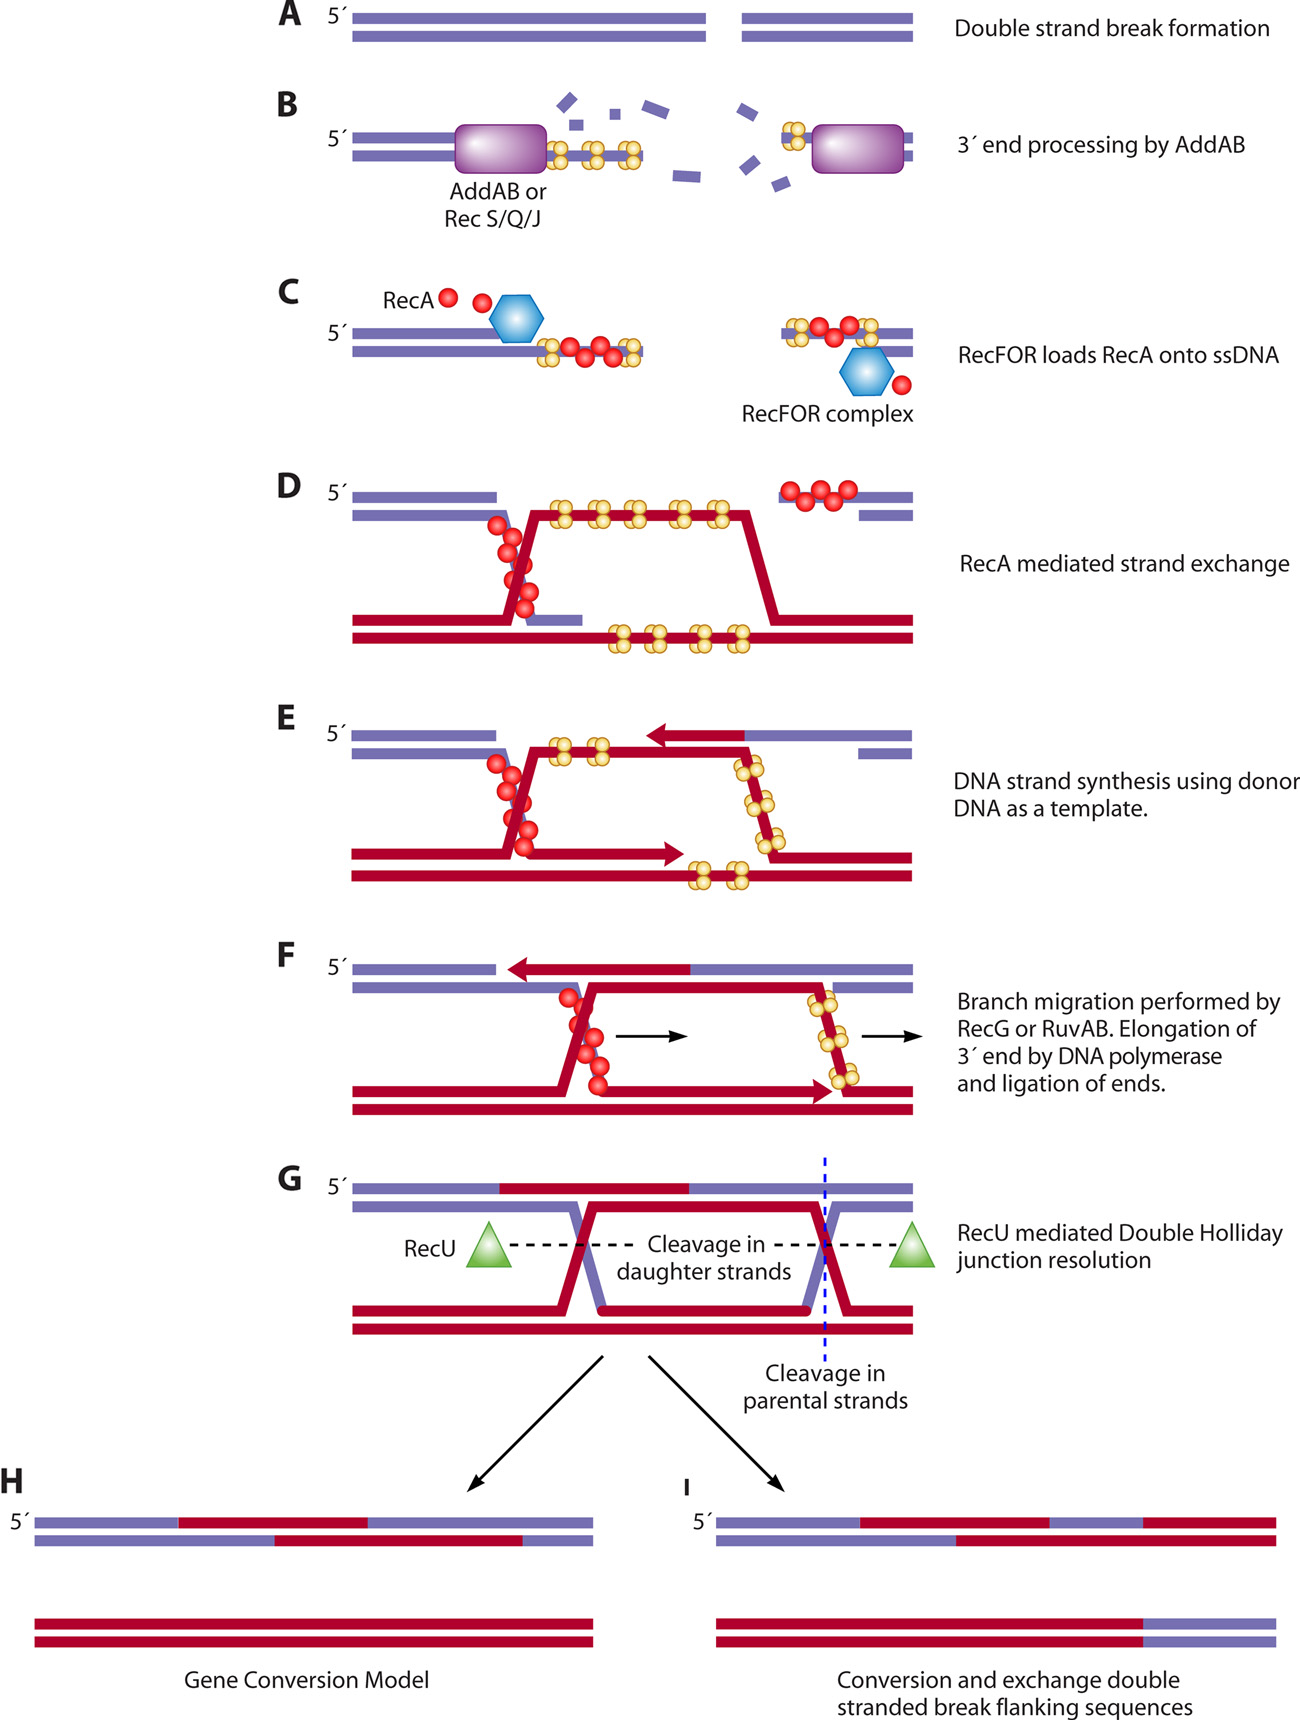
\includegraphics[width=0.54\linewidth]{figure/HR1}
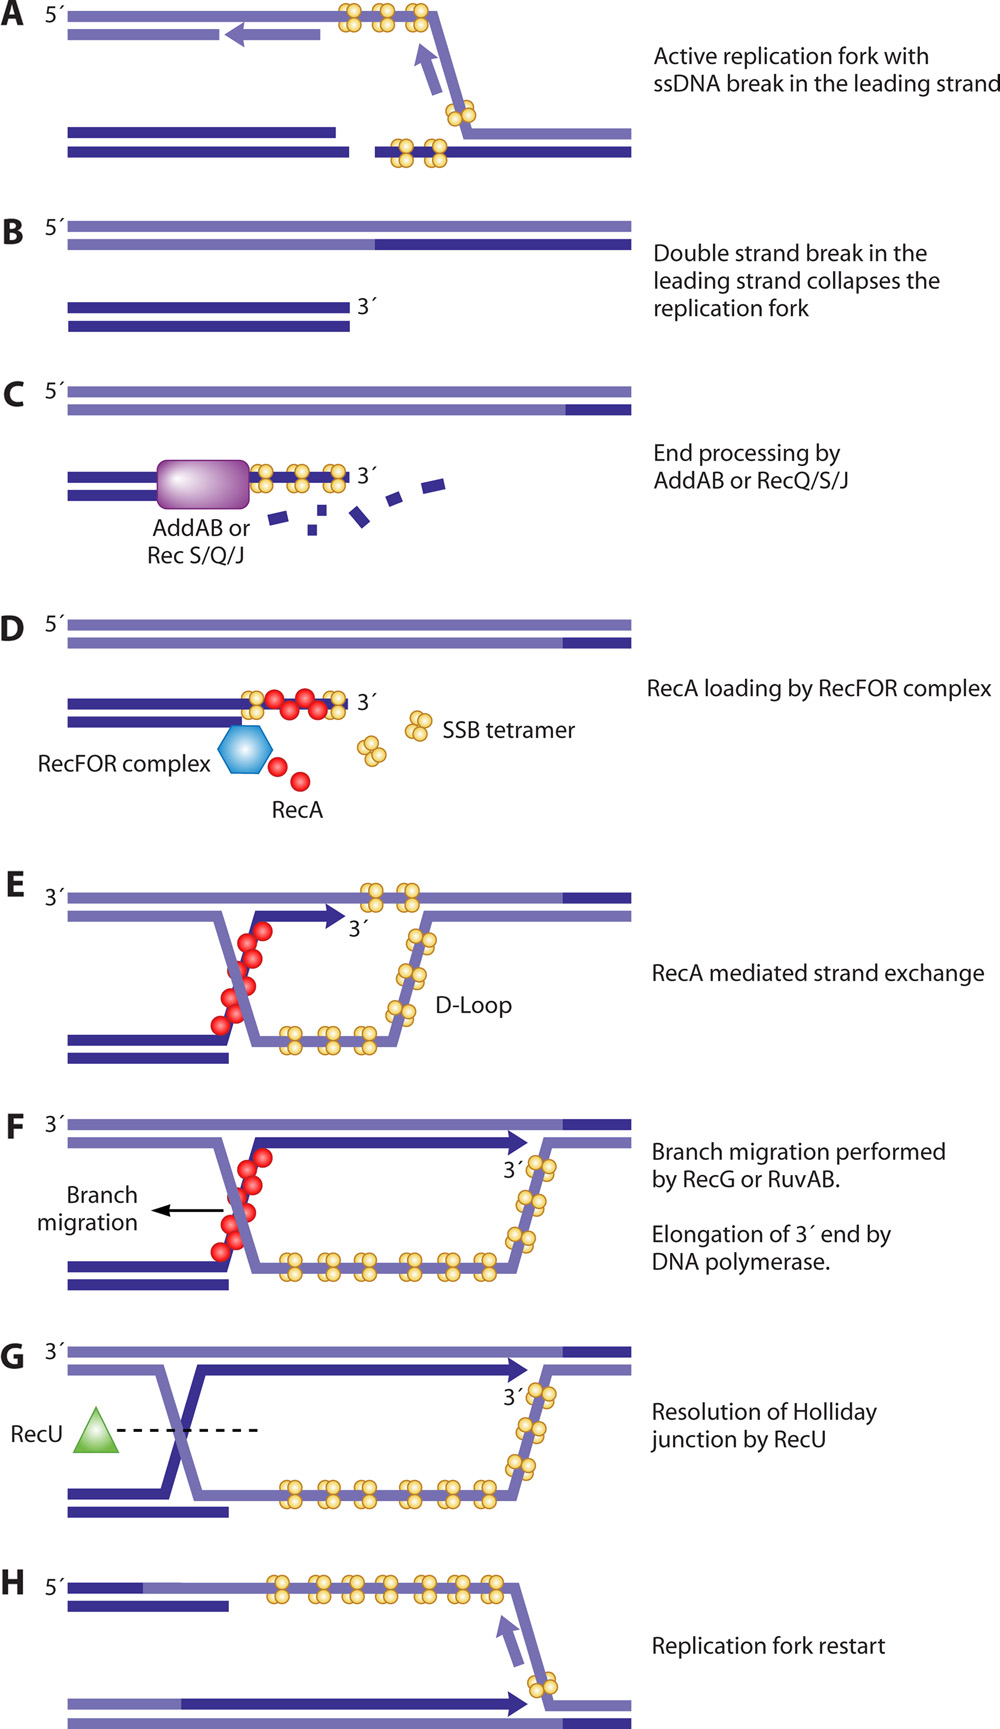
\includegraphics[width=0.44\linewidth]{figure/HR2}
\caption{Homologous recombination and repair of DSB in \textit{B. subtilis} in the general case (left) and when the DSB appears in the replication fork (right). From Lenhart \textit{et al.}.}
\label{fig:HR}
\end{figure}

\subparagraph{Nonhomologous end joining (NHEJ)} This pathway is also responsible for DSB repairing but it is less efficient than homologous recombination. It is used when there is no other copy of the chromosome present in the cell. As in HR, a protein (probably YkoV for \textit{B. subtilis}) binds the DSB and favors recruitment of another protein (LigD like, probably YkoU for \textit{B. subtilis}) that is able to perform exonucleation, polymerisation and ligation. The mechanisms are not totally clear but it seems that because LigD is able to perform these 3 functions, no other protein is needed. However, some bases need to be deleted and repolymerized during the reparation, possibly leading to DNA losses or insertions, making NHEJ a low-fidelity repair mechanism.


\subsubsection{DNA compaction}
\textcolor[rgb]{1.00,0.00,0.00}{Condensation, ”clamping” of the DNA by structural maintenance of chromosome (SMC) proteins, supercoiling, macromolecular crowding, charge neuralization?}
If spatialization is used, condensation and segragation might be modelled directly. Supercoiling needs another state.
\textcolor[rgb]{1.00,0.00,0.00}{Compactation should also impact the accessibility of the chromosome.}

\subsubsection{DNA segregation}
As replication proceeds, sister chromosomes/plasmids have to be separated in order to allow proper cell division. This process is also largely unknown, but several models based on experiments have been proposed, it seems that there is no universal solution valid for all bacteria. There are two main challenges: unlinking the chromosomes and driving them to opposite poles of the cell.

Unlinking is generally done at the replisome level. Supercoiling accumulates at the front of the helicase due to its unwinding activity. This supercoiling can be physically propagated to the back of the replisome, creating an entanglement between sister chromosomes. The DNA gyrase limits this propagation by diminishing supercoiling at the front of the replisome, while Topoisomerase IV disentangles the chromosome copies \citep{reyes-lamothe_chromosome_2012}.

Segregation can be done according to several mechanisms, particularly for plasmids. For high copy number plasmids, it is possible that segregation occurs purely through diffusion. For other plasmids, elements of the cytoskeleton can be used to separate the copies (Figure \ref{fig:dnaMigration}ab). ParR proteins may bind to \textit{parC} loci on the plasmid and serve as a basis for actin-like ParM that polymerizes between the copies, progressively seperating them. Similarly, TubR might bind to \textit{tubC} and migrate along filaments of tubulin-like TubZ. The last mechanism may target plasmids as well as the chromosomes (Figure \ref{fig:dnaMigration}c). It is also composed of a DNA binding protein ParB, binding to \textit{parS} (close to \textit{oriC}), and a motor protein ParA. However, ParA attracts ParB only in its activated and DNA-binding form ParA-ATP, probably forming filaments along the nucleoid. ParB hydrolises ParA-ATP, releasing it in the cytosol until it gets reactivated and rebinds DNA away from ParB. In this way the two ParB-\textit{parS}-\textit{oriC} complexes migrate in opposite directions until steady-state is reached, with equivalent ParA-ATP pools located on each side of each complex (approximately at the quarter of each pole). It seems that this system works cooperatively with SMC proteins, but the details are yet unknown \citep{reyes-lamothe_chromosome_2012} 
\begin{figure}[!ht]
	\centering
	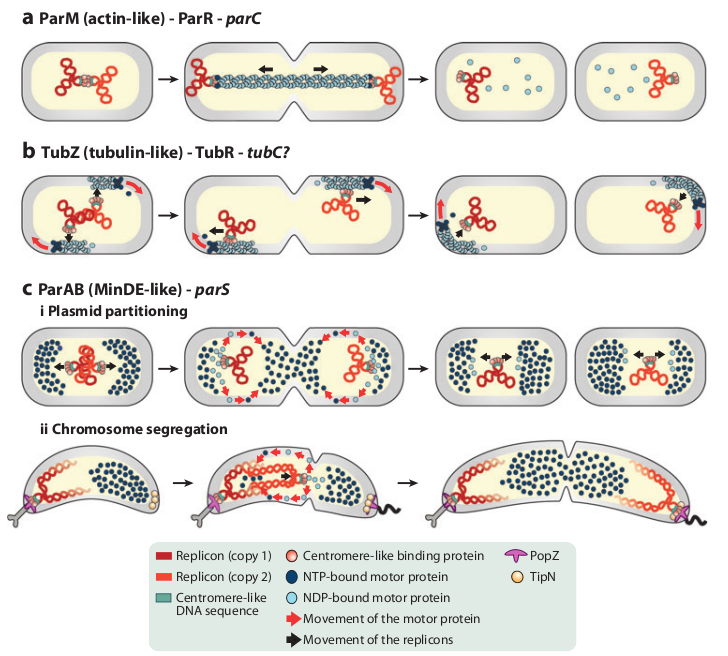
\includegraphics[width=0.8\linewidth]{figure/DNAmigration}
	\caption{Migration of plasmids and chromosome can be mediated by different systems. It can be based on elements of the cytoskeleton: separation through polymerization of actin-like proteins (a), migration along tubulin-like proteins (b). Alternatively, migration may based on an oscillatory system, where activated proteins (ParA-ATP) attracts another protein (ParB) linked to the plasmid or chromosome (\textit{parS} loci) that hydrolises it (c). DNA migration is then controlled by the location of pools of activated proteins. Figure from \citet{reyes-lamothe_chromosome_2012}.}
	\label{fig:dnaMigration}
\end{figure}

Similar to initial segregation, final segregation includes decatanation of two chromosomes and migration of the \textit{ter} region to the two poles, but it is assisted by a new protein and associated with the formation of the FtsZ ring at the septum. The FtsZ ring cannot polymerize as long as the nucleoid is located at the center of the cell. Cytokinesis thus begins when the initial migration of DNA copies is already advanced. Once FtsZ ring forms, the DNA translocase FtsK (SftA in \textit{B. subtilis}) is recruited by the divisome to the membrane next to the FtsZ ring. FtsK seems to coordinate several actions in the final segregation. FtsK binds to \textit{dif} loci next to the \textit{ter} regions, aligning the \textit{ter} region with the septum. FtsK can also translocate remaining DNA at the final stages of septum closing. FtsK also cooperates with Xer proteins to separate chromosomes copies that might have merged due to recombination by creating a Holliday junction.
 

\subsubsection{DNA transformation}

\textcolor{red}{What processes are involved?}
\textcolor{red}{What about plasmid integration, exchange and replication???}
